\section{Umsetzung des Lösungsweges}
\label{sec:umsetzung}

\subsection{Decodierung der STEP-Datei}

Aus dem in Abschnitt \ref{sec:eingabegeometrie} beschriebenen zeilenweisen Aufbau einer STEP-Datei lassen sich die STEP-Entitäten in Java abbilden. Jede Zeile beschreibt genau eine Entität. Diese sind stets nach dem folgenden Muster aufgebaut:

\begin{lstlisting}[captionpos=b, style=customc, caption=Beschreibung eines Punktes in STEP, label=lst:simplestp]
#ID=KLASSE(ATTRIBUTSLISTE);
\end{lstlisting}

Aufgrund dieses einheitlichen Musters lassen sie sich relativ einfach dekodieren und als Java-Klassen in Programmcode umwandeln um in einem weiteren Schritt die Struktur des Bauteils abzubilden.
Das Ziel des ersten Schrittes in der Lösungsumsetzung besteht nun darin, aus einer einzelnen Zeile der STEP-Datei Java-Objekte zu bilden und mit den Daten aus der jeweiligen Zeile zu belegen.    

\subsubsection{Implementierte STEP-Entitäten}

Die verschiedenen Entitätstypen, die in einer STEP-Datei vohanden sein können sind in der STEP-Dokumentation [Referenz einfügen] aufgeführt. Die Attribute, welche zu jeder einzelnen Klasse gehören werden darin beschrieben.
Da die Implementierung aller vorhandenen STEP-Klassen den Rahmen dieser Arbeit überschreiten würde, sind vorerst folgende Klassen im Programm umgesetzt. Es ist anzumerken, dass nicht jede Klasse eine Instanz bilden kann. Diese sogenannten abstrakten Klassen dienen zur Gruppierung von sich ähnlichen nicht abstrakten Klassen. Diese sind Bestandteil des Vererbungsprinzips der objektorientierten Programmierung in Java. Sie sind in der Liste als solche gekennzeichnet.  
\begin{itemize}
	\item REPRESENTATION\_ITEM (abstrakt)
	\item GEOMETRIC\_REPRESENTATION\_ITEM (abstrakt)
	\item TOPOLOGICAL\_REPRESENTATION\_ITEM (abstrakt)
	\item POINT (abstrakt)
	\item CARTESIAN\_POINT
	\item DIRECTION
	\item VECTOR
	\item PLACEMENT (abstrakt)
	\item AXIS2\_PLACEMENT\_3D
	\item SURFACE (abstrakt)
	\item ELEMENTARY\_SURFACE (abstrakt)
	\item PLANE
	\item CYLINDRICAL\_SURFACE	
	\item CURVE (abstrakt)
	\item LINE
	\item CONIC (abstrakt)
	\item CIRCLE 
	\item VERTEX (abstrakt)
	\item VERTEX\_POINT
	\item EDGE (abstrakt)
	\item EDGE\_CURVE
	\item ORIENTED\_EDGE
	\item LOOP (abstrakt)
	\item EDGE\_LOOP
	\item FACE\_BOUND
	\item OUTER\_FACE\_BOUND
	\item FACE (abstrakt)
	\item FACE\_SURFACE
	\item ADVANCED\_FACE
\end{itemize}

\subsubsection{Erläuterung der implementierten STEP-Entitäten}

\paragraph{CARTESIAN\_POINT}

Beschreibt einen Punkt im dreidimensionalen Raum mit den Koordinaten x, y und z (in mm) bezogen auf das Weltkoordinatensystem des in der STEP-Datei beschriebenen Bauteils. Diese Punkte dienen als Basis für viele weitere STEP-Entitäten, beziehen sich selbst aber nicht auf andere Objekte. 

\paragraph{DIRECTION}

Ebenso wie die CARTESIAN\_POINTs beziehen sich diese Entitäten nicht auf andere. Sie repräsentieren einen normalisierten Richtungsvektor (Länge = 1mm) mit den Richtungskoordinaten x, y, z (in mm). Diese Richtungsvektoren werden von vielen STEP-Entitäten referenziert.

\paragraph{VECTOR}

Stellt einen räumlichen Vektor dar. Dieser hat als Grundgeometrie einen normalisierten Richtungsvektor (DIRECTION) und eine gegebene Länge. Ein VECTOR bezieht sich demnach, anders als die vorher beschriebenen Klassen auf ein Objekt einer anderen Klasse.

\paragraph{AXIS2\_PLACEMENT\_3D}

Beschreibt ein lokales Koordinatensystem im Raum. Es besteht aus einem CARTESIAN\_POINT, welcher die Position des lokalen Koordiantenursprunges darstellt. Des Weiteren definieren zwei Richtungsvektoren die Ausrichtung dieses lokalen Koordinatensystems.

\paragraph{LINE}

Beschreibt eine gerade Strecke im Raum. Eine LINE wird gebildet aus einem CARTESIAN\_POINT, welcher den Startpunkt der Linie darstellt sowie einem VECTOR, welcher Richtung und Länge der Strecke bestimmt. 

\paragraph{CIRCLE}

Definiert einen Kreis im dreidimensionalen Raum. Die Position (Mittelpunkt) und Ausrichtung des Kreises wird durch ein lokales Koordinatensystem in Form eines AXIS2\_PLACEMENT\_3D beschrieben. Dabei steht der erste Vektor des lokalen Koordinatensystems senkrecht auf der Ebene, in welcher der Kreis liegt. Der zweite Vektor liegt in der Kreisebene. Abbildung \ref{fig:circleentity} verdeutlicht den Aufbau. 

\begin{figure}[h]
	\centering
	
	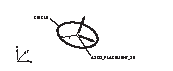
\includegraphics[width=0.7\linewidth]{img/circle_entity.pdf}
	
	
	\caption{Visualisierung CIRCLE}
	\label{fig:circleentity}
\end{figure} 

\paragraph{PLANE}

Beschreibt eine Ebene im Raum. Diese Ebene hat keine räumliche Begrenzung und ist durch einen AXIS2\_PLACEMENT\_3D eindeutig definiert. Ähnlich wie beim CIRCLE legt der erste Vektor des lokalen Koordinatensystems den Normalenvektor der Ebene fest. Der zweite Vektor beschreibt einen Richtungsvekotor der Ebene. Durch den Koordinatenursprung des lokalen Koordinatensystems, wird der Ortsvektor der Ebene definiert. 

\begin{figure}[h]
	\centering
	
	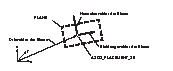
\includegraphics[width=0.7\linewidth]{img/plane_entity.pdf}
	
	
	\caption{Visualisierung PLANE}
	
\end{figure} 

\paragraph{CYLINDRICAL\_SURFACE}


Beschreibt analog zur PLANE eine zylindrische Ebene im Raum. Diese kann man sich vorstellen als Mantelfläche eines unendlich langen Zylinders. Die Lage des Zylinders wird auch hier durch eine AXIS2\_PLACEMENT\_3D definiert und hat als zusätzlichen Parameter eine Zahlenwertangabe zum Radius. In der folgenden Abbildung ist zu erkennen, dass die Achse des Zylinders aus dem ersten Vektor des lokalen Systems gebildet wird und der zweite Vektor in der parallel zur Deckfläche des Zylinders liegt.

\begin{figure}[h]
	\centering
	
	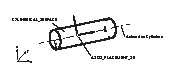
\includegraphics[width=0.7\linewidth]{img/cylinder_entity.pdf}
	
	\caption{Visualisierung CYLINDRICAL\_SURFACE}
	
\end{figure}

\paragraph{VERTEX\_POINT}

Definiert einen Punkt des Bauteils im Raum. Dieser wird definiert durch einen CARTESIAN\_POINT. Der Unterschied diesem besteht darin, dass es sich bei einem VERTEX\_POINT um einen tatsächlichen Punkt des Bauteils (beispielsweise ein Eckpunkt einer Körperkante) handelt und nicht um eine bloße Referenz.   

\paragraph{EDGE\_CURVE}

Beschreibt eine Körperkante. Dabei kann es sich um verschiedene Kantentypen, wie Kreise, Linien oder Splines  handeln. Definiert werden Anfangs- und Endpunkt der EDGE\_CURVE. Diese werden als Körperpunkte (VERTEX) definiert. Handelt es sich um eine geschlossene Kante, beispielsweise einen Kreis, dann sind Anfangs- und Endvertex identisch. Außerdem weißt eine EDGE\_CURVE eine Orientierung auf. Diese wird durch einen boolschen Wert (wahr oder falsch) angegeben und definiert so eindeutig Anfangs- bzw. Endpunkt der Körperkante.   

\paragraph{EDGE\_LOOP}

Beschreibt einen Kantenverbund aus mehreren Körperkanten. Dieser Kantenverbund ist geschlossen und erhält als Parameter die Liste der enthaltenen Körperkanten. 

\paragraph{FACE\_OUTER\_BOUND}

Beschreibt die äußere Umrandung einer Körperfläche und wird durch eine EDGE\_LOOP beschrieben. Dies kann zum Beispiel ein Polygon aus verschiedenen Linien oder Kurvenstücken sein. Solch eine äußere Umrandung kann aber auch durch einen Kreis definiert sein.

\paragraph{FACE\_BOUND}

Defininert die innere Umrandung einer Körperfläche eine EDGE\_LOOP beschrieben. Dies kann, wie bei einer FACE\_OUTER\_BOUND, durch ein Polygon aus verschieden Linien oder Kurvenstücken sein. Solch eine äußere Umrandung kann aber auch durch einen Kreis definiert sein.   

\paragraph{ADVANCED\_FACE}

Beschreibt eine tatsächliche Körperfläche des in der STEP-Datei formulierten Bauteils. Definiert ist die Fläche zum einen durch eine Liste an Umrandungen(BOUNDs) und durch die Angabe einer PLANE bzw. CYLINDRICAL\_SURFACE in welcher diese Umrandungen liegen. Diese Körperflächen sind in ihrer räumlichen Ausdehnung begrenzt. Die Menge aller ADVANCED\_FACES einer STEP-Datei ergeben zusammengesetz das beschriebene Modell des Bauteils. 

Abbildung \ref{fig:advancedfaceentity} zeigt den Aufbau einer planaren ADVANCED\_FACE aus einer äußeren Umrandung in Form eines Polygons (EDGE\_LOOP aus mehreren LINE-Entitäten) und einer inneren Umrandung durch einen Kreis.  

\begin{figure}[h]
	\centering
	
	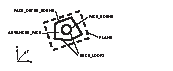
\includegraphics[width=0.7\linewidth]{img/advancedface_entity.pdf}
	
	\caption{Visualisierung planare ADVANCED\_FACE}
	\label{fig:advancedfaceentity}
	
\end{figure}

\subsubsection{Bildung einzelner STEP-Entitäten}
\label{sec:string2entity}


Nach der Eingrenzung der zu realisierenden STEP-Entitäten und der Erklärung dieser folgt in diesem Abschnitt die Beschreibung, wie aus einer Zeile der STEP-Datei eine konkretes Java-Objekt gebildet wird. 

Zuerst müssen alle impelementierten STEP-Entitäten als Java-Klassen beschrieben werden. Diese dienen als Muster für die verschiedenen Objekte der STEP-Datei. Die oben aufgeführten Klassen sind im Projektordner \textit{"`./src/main/java/com.jandoant/stp\_entities"'} zu finden. Diese enthalten die entsprechend der STEP-Dokumentation aufgeführten Attribute für jede Entität. 

In der Klasse \textit{StpEntityBuilder} im Projektordner \textit{"`./src/main/java/com.jandoant/builder"'} wird dies umgesetzt. Diese Klasse wird im Programmablauf für jede Zeile der STEP-Datei einmal aufgerufen. Übergeben wird ihr die Zeichenkette der jeweiligen Zeile. Aus dieser übergebenen Zeichenkette kann die Klasse nun, mit Aufruf der Funktion \textit{extractStpEntity()} ein entsprechendes Objekt der beschriebenen STEP-Entität bilden. 
Dazu wird die beschreibende Zeichenkette in ihre drei Bestandteile (ID, Klassenname, Attibutsliste) zerlegt. Über die Kenntnis des Klassennamens, kann die Klasse \textit{StpEntityBuilder} entscheiden, welcher Entitätstyp erzeugt werden soll. In einem weiteren Schritt wird die Elemente der Attributsliste extrahiert und ein konkretes Java-Objekt einer STEP-Entität mit all seinen konkreten Attributen kann gebildet werden. Es ist aber festzuhalten, dass es zu diesem Zeitpunkt noch nicht möglich ist, die tatsächlichen Referenzobjekte in der erzeugten Entität festzuhalten. Vorerst kann aus der Zeichenkette nur die jeweilige ID der Referenzobjekte gespeichert werden. Die Zuordnung kann erst von statten gehen, wenn alle Zeilen der STEP-Datei in Java-Objekte ausgelesen wurden.

\subsubsection{Abbildung des gesamten STEP-Modells in Java} 

Das Programm ist, wie im vorherigen Abschnitt gezeigt in der Lage, aus einer einzelnen Zeile der vorliegenden STEP-Datei ein konkretes Java-Objekt zu extrahieren. Nun folgt in diesem Schritt die Decodierung der gesamten Datei. Nach Beendigung dieses Vorgangs ist die komplette geometrische Bauteilstruktur im Programm abgebildet und kann darauffolgend weiterverarbeitet werden.

Der Vorgang dieser Decodierung erfolgt durch die Klasse \textit{StpModelBuilder}, welche sich im Projektordner \textit{"`./src/main/java/com.jandoant/builder"'} befindet. 
Wird diese Klasse im Programmablauf instantiiert, so wird ihr der absolute Pfad, unter dem die zu verarbeitende STEP-Datei liegt übergeben. Mit dieser Information hat die erzeuge Instanz den Zugriff auf alle Zeilen der Datei, welche die Bauteilgeometrie beschreiben.
Mit Aufruf der Funktion \textit{parseFile()} wird die übergebene STEP-Datei verarbeitet. Dabei werden zunächst alle Zeilen der Datei durchlaufen. Jede Zeichenkette, die eine STEP-Entität beschreibt, also mit dem \#-Symbol beginnt und mit einem Semikolon endet, wird in einer Liste dieser Zeichenketten zwischengespeichert. Es ist dabei unerheblich, ob die Zeichenkette durch einen oder mehrere Zeilenumbrüche getrennt ist. Dies hat den Effekt, dass die HEADER-Sektion herausgefiltert wird. Diese hat keine Bedeutung für die grundlegende Funktion des Programms, da in diesem Abschnitt der Datei keine STEP-Entitäten beschrieben werden.

Aus der erzeugten Liste an Zeichenketten, welche dem gewünschten Muster entsprechen, werden im folgenden Bearbeitungsschritt unter Anwendung der in \prettyref{sec:string2entity} dargelegten Methode  der Klasse  \textit{StpEntityBuilder} die jeweilig beschriebenen STEP-Entitäten im Java-Code instantiiert und in einer List zwischengespeichert. Dabei ist anzumerken, dass ausschließlich die in der Klasse "`StpEntityContract"' im Projektordner \textit{"`./src/main/java/com.jandoant/stp\_entities"'} festgehaltenen STEP-Entitäten decodiert werden. Alle Zeichenketten, die nicht eine solche Entität beschreiben, werden ignoriert. Das führt dazu, dass ausschließlich die geometrischen Informationen des Modells extrahiert werden. Andere Angaben, die in der STEP-Datei festgehalten sein können, werden bei dieser Implementierung nicht berücksichtigt, da sie für die grundlegende Funktion des Programmes unerheblich sind.

Nach dem Durchlaufen aller Zeilen und anschließender Instanziierung der Java-Objekte entsprechend der STEP-Beschreibung, liegt zu diesem Punkt eine Liste mit allen vorkommenden geometrischen STEP-Entitäten im Programm vor. Allerdings ist damit den Anforderungen noch nicht entsprochen. Nach der Decodierung der einzelnen Zeichenketten haben die Java-Objekte noch keine Relation zueinander. Wie in \prettyref{sec:string2entity} erläutert, sind die Referenzentitäten, auf die sich eine STEP-Entität bezieht, bisher nur mit ihrer ID-erfasst. Eine Zuordnung der Objekte passiert nun aus vorliegender Liste der erzeugten Java-Objekte. 
Dazu wird die Methode \textit{convertFromIds()} aufgerufen, welche in jeder Java-Klasse, die eine STEP-Entität beschreibt, implementiert ist.
Mit Aufruf der Methode durch das betreffende Java-Objekt wird die Entitätsliste durchlaufen. Dabei werden alle Entitäten, deren ID mit einer der IDs, die in diesem Java-Objekt hinterlegt sind, herausgefiltert und dem Java-Objekt zugewiesen. Nachdem dieser Vorgang für alle Objekte der Liste ausgeführt wurde, sind alle Referenzen über tatsächliche Java-Objekte hergestellt. 

Die im Programmablauf aufgerufene Methode \textit{parseFile()} der Klasse \textit{StpModelBuilder} gibt nun in einem finalen Schritt alle \textit{ADVANCED\_FACE}s, die in der STEP-Datei durch Zeichenketten beschrieben wurden, als tatsächliche Java-Objekte an das Programm zurück. Dies geschieht in Form einer Liste.  Diese \textit{ADVANCED\_FACE}s  referenzieren wie oben beschrieben alle Objekte, durch welche sie selbst definiert werden. Somit ist die gesamte Bauteilstruktur im Programm abgebildet und kann im weiteren Ablauf des Programms verarbeitet werden.

\subsection{Diskretisierung der Körperflächen}

Um die Diskretisierung der Oberflächen zu realisieren wird über eine Änderung des Koordinatensystems realisiert. Ziel ist dabei die Umwandlung Punkte der Körpfläche in ein lokales flächenorientiertes Koordinatensystem (Mapping). Dabei werden alle Punkte der jeweiligen Fläche einer Koordinatentransformation unterzogen. So besitzt jeder Punkt eine Beschreibung im Weltkoordinatensystem mit Werten in x, y und z-Richtung. Gleichzeitig gelten aber für ebendiesen Punkt auch Definitionen bezüglich des lokalen Koordinatensystems in u-, v- und w-Richtung. Die folgende Abbildung verdeutlicht dies.
 
\subsubsection{Basistransformation}

Um eine Basistransformation zwischen Welt- und lokalem Koordinatensystem durchführen zu können ist es notwendig, sowohl die Einheitsbasisvektoren des Weltkoordinatensystem, als auch die des lokalen Systems zu kennen. Die Einheitsbasisvektoren des Weltkoordiantensystems sind stets die selben und werden wie folgt definiert:

\begin{singlespace}
\begin{equation}
\begin{aligned}
\vv{e_{x}}=\begin{pmatrix}
1 \\ 
0 \\ 
0
\end{pmatrix}  
&& 
\vv{e_{y}}=\begin{pmatrix}
0 \\ 
1 \\ 
0
\end{pmatrix}  
&& 
\vv{e_{z}}=\begin{pmatrix}
0 \\ 
0 \\ 
1
\end{pmatrix} 
\end{aligned}
\end{equation}
\end{singlespace}

Die Menge aller Punkte einer Ebene wird in der Geometrie durch die Formel

\begin{equation}
E: \vv{x} = \vv{x_{0}} + r \cdot \vv{x_{R1}} + s \cdot \vv{x_{R2}}  
\end{equation}

eindeutig definiert. Dabei steht $\vv{x}$ für einen beliebigen Punkt der Ebene. $\vv{x_{0}}$ beschreibt den Ortsvektor, $\vv{x_{R1}}$ und $\vv{x_{R2}}$  die Richtungsvektoren und $r$ und $s$ beliebige Laufparameter um die Lage des Punktes als Linearkombination dieser Vektoren genau zu beschreiben.

Die Basiseinheitsvektoren $\vv{e_{u}}$, $\vv{e_{v}}$ und $\vv{e_{w}}$ des lokalen Koordinatensystems werden aus der \textit{AXIS2\_PLACEMENT\_3D} des Flächenelementes gebildet, auf dem die \textit{ADVANCED\_FACE} liegt. Die erste \textit{DIRECTION} der \textit{AXIS2\_PLACEMENT\_3D} entspricht dem Normalenvektor der Ebene, die zweite \textit{DIRECTION} einem Richtungsvektor.

Bei ebenen Flächen sind dies die beiden normalisierten Richtungsvektoren der Ebene, auf der sie liegen. Der Koordinatenursprung liegt in dem Punkt, der durch den Ortsvektor $\vv{x_{0}}$ der Ebene beschrieben wird. In der \textit{AXIS2\_PLACEMENT\_3D} des Flächenelementes sind aber nur der Normalenvektor $\vv{n}$ der Ebene und ein Richtungsvektor beschrieben. Der fehlende Richtungsvektor wird durch die Bildung des Kreuzproduktes der beiden für ein rechtshändiges System nach \prettyref{eq:crossproduct} erzeugt.

\begin{equation}\label{eq:crossproduct}
	\vv{x_{R2}} = \vv{n} \times \vv{x_{R1}}
\end{equation}

Die Basisvektoren des lokalen Systems können somit entsprechend \prettyref{eq:basevectorsuvw}  gebildet werden.

\begin{equation}\label{eq:basevectorsuvw}
	\begin{aligned}
	\vv{e_{u}}=\vv{x_{R1}} 
	&& 
	\vv{e_{v}}=\vv{x_{R2}}  
	&& 
	\vv{e_{w}}=\vv{x_{n}} 
	\end{aligned}
\end{equation}

Sind die Basiseinheitsvektoren der beiden Koordinatensysteme bekannt, so lassen sich die jeweiligen Basismatrizen  durch spaltenweise Aneinanderreihung der Vektoren bilden. Die Basis des Weltkoordinatensystems ergibt sich damit zur Basismatrix $B_{XYZ}$ nach \prettyref{eq:basematrixxyz}. 

\begin{singlespace}
	\begin{equation}\label{eq:basematrixxyz}
		B_{XYZ} = \begin{pmatrix}
		1 & 0 & 0 \\ 
		0 & 1 & 0 \\ 
		0 & 0 & 1
		\end{pmatrix} 
	\end{equation} 
\end{singlespace}

Die Basis des Weltkoordinatensystems ergibt sich analog zur Basismatrix $B_{UVW}$ nach \prettyref{eq:basematrixuvw}.

\begin{singlespace}
	\begin{equation}\label{eq:basematrixuvw}
	B_{UVW} = \begin{pmatrix}
	e_{u_x} & e_{v_x} & e_{w_x} \\ 
	e_{u_y} & e_{v_y} & e_{w_y} \\ 
	e_{u_z} & e_{v_z} & e_{w_z}
	\end{pmatrix} 
	\end{equation} 
\end{singlespace}

Die Transformationsmatrix um einen Punkt vom globalen in das lokale Koordinatensystem der Ebene zu transformieren ergibt sich nach \prettyref{eq:trafoXYZ2UVW}.

\begin{equation}\label{eq:trafoXYZ2UVW}
T_{XYZ \rightarrow UVW} = B_{UVW}^{-1} \cdot B_{XYZ}  
\end{equation}   

Die Transformationsmatrix um einen Punkt wieder aus dem lokalen Koordinatensystem der Ebene zurück in das globale System zu transformieren ergibt sich nach \prettyref{eq:trafoUVW2XYZ} aus der Inversen der Transformationsmatrix aus \prettyref{eq:trafoXYZ2UVW}.

\begin{equation}\label{eq:trafoUVW2XYZ}
T_{UVW \rightarrow XYZ} = T_{XYZ \rightarrow UVW}^{-1} 
\end{equation}   



\subsubsection{Diskretisierung zylindrischer Flächen}

\subsubsection{Diskretisierung planarer Flächen}

\subsection{Deformation der Körperflächen}

\subsection{Ausgabe der verformten Geometrie}





           


       

        








    













  
